\documentclass{beamer}
\usepackage[utf8]{inputenc}
\usepackage{graphicx, epsfig}
\usepackage{amsmath,mathrsfs,amsfonts,amssymb}
\usepackage{floatflt}
\usepackage{epic,ecltree}
\usepackage{mathtext}
\usepackage{fancybox}
\usepackage{fancyhdr}
\usepackage{multirow}
\usepackage{enumerate}
\usepackage{epstopdf}
\usepackage{multicol}
\usepackage{algorithm}
\usepackage[noend]{algorithmic}
\usepackage{tikz}
\usepackage{blindtext}
\usepackage{multido}
\usetheme{default}%{Singapore}%{Warsaw}%{Warsaw}%{Darmstadt}
\usecolortheme{default}

\setbeamerfont{title}{size=\Huge}
\setbeamertemplate{footline}[frame number]{}

\setbeamertemplate{section in toc}[sections numbered]

\makeatletter
\newcommand\HUGE{\@setfontsize\Huge{35}{40}}
\makeatother    

\setbeamerfont{title}{size=\HUGE}
\beamertemplatenavigationsymbolsempty

\usetikzlibrary{arrows,shapes,positioning,shadows,trees}

\newcommand\myfootnote[1]{%
  \vspace{-0.5cm}%
  \tikz[remember picture,overlay]
  \draw (current page.south west) +(1in + \oddsidemargin,0.5em)
  node[anchor=south west,inner sep=0pt]{\parbox{\textwidth}{%
      \rlap{\rule{10em}{0.4pt}}\raggedright\scriptsize \textit{#1}}};}

\newcommand\myfootnotewithlink[2]{%
  \vspace{-0.5cm}%
  \tikz[remember picture,overlay]
  \draw (current page.south west) +(1in + \oddsidemargin,0.5em)
  node[anchor=south west,inner sep=0pt]{\parbox{\textwidth}{%
      \rlap{\rule{10em}{0.4pt}}\raggedright\scriptsize\href{#1}{\textit{#2}}}};}

\AtBeginSection[]
      {
      	\begin{frame}{Outline}
      		\tableofcontents[currentsection]
      	\end{frame}
      }
      \AtBeginSubsection[]{
      	\begin{frame}{Outline}
      		\tableofcontents[currentsection,currentsubsection]
      	\end{frame}
}

\newcounter{noscounter} % Используется для nextonslide команды (обнуляется только на новом слайде)
\newcounter{pcounter} % Используется для pause команды (обнуляется после использования eqpause)
\newcounter{diffcounter} % Считает количество pause после формулы

\newcommand{\nextonslide}[1]{%
  \stepcounter{noscounter}% Прибавляем счетчик nextonslide
  \stepcounter{pcounter}% Прибавляем счетчик pause
  \stepcounter{diffcounter}% Прибавляем счетчик diffcounter
  \onslide<\value{noscounter}->{#1}% Отображаем аргумент в скобках на слайде с номером noscounter
}
\newcommand{\resetonslide}{%
    \setcounter{noscounter}{1}% Сбрасываем счетчик nextonslide
    \setcounter{pcounter}{1}% Сбрасываем счетчик pause
    \setcounter{diffcounter}{0}% Сбрасываем счетчик diffcounter
}

\newcommand{\eqpause}{%
  \multido{\i=1+1}{\value{pcounter}}{\pause}% Повторяем pcounter раз команду pause
  \stepcounter{noscounter}% Прибавляем счетчик nextonslide
  \setcounter{pcounter}{1}% Сбрасываем счетчик pause
}

\newcommand{\eqpausediff}{% Вспомогательная команда, запускается автоматически после формул
  \multido{\i=1+1}{\value{diffcounter}}{\pause}% Повторяем diffcounter раз команду pause
  \addtocounter{pcounter}{-\value{diffcounter}}% Вычитаем из pcounter количество сделанных pause
  \setcounter{diffcounter}{0}% Сбрасываем счетчик diffcounter
}

\newcommand\AtEndBoth[2]{% Применяем команду к multline и multline*
  \AtEndEnvironment{#1}{#2}%
  \AtEndEnvironment{#1*}{#2}%
}

\AtEndBoth{align}{\eqpausediff}
\AtEndBoth{equation}{\eqpausediff}
\AtEndBoth{multline}{\eqpausediff}

\addtobeamertemplate{frametitle}{\resetonslide}{}% На каждом слайде сбрасываем счетчики

% latin bold lower
\newcommand{\ba}{\mathbf{a}} 
\newcommand{\bc}{\mathbf{c}} 
\newcommand{\be}{\mathbf{e}} 
\newcommand{\bff}{\mathbf{f}} % \bf - for bold type
\newcommand{\bg}{\mathbf{g}} 
\newcommand{\bh}{\mathbf{h}} 
\newcommand{\bp}{\mathbf{p}} 
\newcommand{\bq}{\mathbf{q}} 
\newcommand{\bt}{\mathbf{t}} 
\newcommand{\bs}{\mathbf{s}} 
\newcommand{\bu}{\mathbf{u}} 
\newcommand{\bv}{\mathbf{v}} 
\newcommand{\bw}{\mathbf{w}} 
\newcommand{\bx}{\mathbf{x}} 
\newcommand{\by}{\mathbf{y}} 
\newcommand{\bz}{\mathbf{z}} 

% latin bold upper
\newcommand{\bA}{\mathbf{A}} 
\newcommand{\bB}{\mathbf{B}} 
\newcommand{\bC}{\mathbf{C}} 
\newcommand{\bG}{\mathbf{G}} 
\newcommand{\bI}{\mathbf{I}} 
\newcommand{\bJ}{\mathbf{J}} 
\newcommand{\bL}{\mathbf{L}} 
\newcommand{\bM}{\mathbf{M}} 
\newcommand{\bP}{\mathbf{P}}
\newcommand{\bQ}{\mathbf{Q}} 
\newcommand{\bR}{\mathbf{R}} 
\newcommand{\bT}{\mathbf{T}} 
\newcommand{\bU}{\mathbf{U}} 
\newcommand{\bV}{\mathbf{V}} 
\newcommand{\bW}{\mathbf{W}} 
\newcommand{\bX}{\mathbf{X}} 
\newcommand{\bY}{\mathbf{Y}} 
\newcommand{\bZ}{\mathbf{Z}} 

% latin cal upper
\newcommand{\cF}{\mathcal{F}} 
\newcommand{\cG}{\mathcal{G}} 
\newcommand{\cI}{\mathcal{I}} 
\newcommand{\cL}{\mathcal{L}} 
\newcommand{\cM}{\mathcal{M}} 
\newcommand{\cN}{\mathcal{N}} 
\newcommand{\cP}{\mathcal{P}} 
\newcommand{\cS}{\mathcal{S}} 
\newcommand{\cT}{\mathcal{T}} 
\newcommand{\cW}{\mathcal{W}} 
\newcommand{\cX}{\mathcal{X}} 
\newcommand{\cZ}{\mathcal{Z}} 

% latin bb upper
\newcommand{\bbE}{\mathbb{E}} 
\newcommand{\bbI}{\mathbb{I}} 
\newcommand{\bbP}{\mathbb{P}} 
\newcommand{\bbR}{\mathbb{R}} 

% greek bold lower
\newcommand{\bepsilon}{\boldsymbol{\epsilon}} 
\newcommand{\btheta}{\boldsymbol{\theta}} 
\newcommand{\blambda}{\boldsymbol{\lambda}} 
\newcommand{\bpi}{\boldsymbol{\pi}} 
\newcommand{\bmu}{\boldsymbol{\mu}} 
\newcommand{\bsigma}{\boldsymbol{\sigma}} 
\newcommand{\bphi}{\boldsymbol{\phi}} 

% greek bold upper
\newcommand{\bSigma}{\boldsymbol{\Sigma}} 

\DeclareMathOperator*{\argmin}{arg\,min}
\DeclareMathOperator*{\argmax}{arg\,max}
\newcommand{\createdgmtitle}[1]{\title[\hbox to 56mm{Deep Generative Models  \hfill\insertframenumber\,/\,\inserttotalframenumber}]
	{\vspace{1cm} \\ \textbf{Deep Generative Models} \\ {\Huge Lecture #1}}
	\author{Roman Isachenko}
	\institute{
		Moscow Institute of Physics and Technology \\
		Yandex School of Data Analysis
	}
	\date{2025, Autumn}
}
\createdgmtitle{14}

\usepackage{tikz}

\usetikzlibrary{arrows,shapes,positioning,shadows,trees}
%--------------------------------------------------------------------------------
\begin{document}
%--------------------------------------------------------------------------------
\begin{frame}[noframenumbering,plain]
%\thispagestyle{empty}
\titlepage
\end{frame}
%=======
\begin{frame}{Outline}
	\tableofcontents
\end{frame}
%=======
\begin{frame}{Recap of Previous Lecture}
    \myfootnotewithlink{https://dl.heeere.com/conditional-flow-matching/blog/conditional-flow-matching}{image credit: A Visual Dive into Conditional Flow Matching}
	\begin{figure}
		\centering
		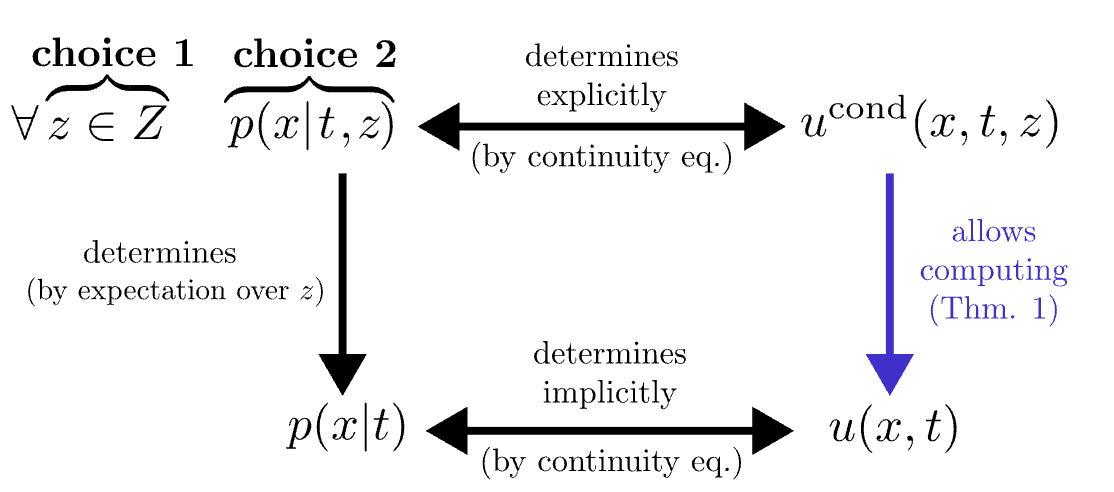
\includegraphics[width=0.7\linewidth]{figs/cfm_uncond_to_cond}
	\end{figure}
	\vspace{-0.3cm}
	\begin{block}{Constraints}
		\vspace{-0.3cm}
		\[
			p(\bx) = \cN(0, \bI) = \bbE_{p(\bz)} p_0(\bx | \bz); \quad \pi(\bx) = \bbE_{p(\bz)} p_1(\bx | \bz).
		\]
		\vspace{-0.5cm}
	\end{block}
	\begin{itemize}
		\item How should we choose the conditioning latent variable $\bz$?
		\item How can we define $p_t(\bx | \bz)$ so that it meets the constraints?
	\end{itemize}
	\begin{block}{Gaussian Conditional Probability Path}
		\vspace{-0.3cm}
		\[
			p_t(\bx | \bz) = \cN\left(\bmu_t(\bz), \bsigma_t^2(\bz)\right)
		\]
		\[
			\bx_t = \bmu_t(\bz) + \bsigma_t(\bz) \odot \bx_0, \quad {\color{violet} \bx_0 \sim p_0(\bx) = \cN(0, \bI)}
		\]
	\end{block}
\end{frame}
%=======
\begin{frame}{Recap of Previous Lecture}
    \myfootnotewithlink{https://arxiv.org/abs/2210.02747}{Lipman Y., et al. Flow Matching for Generative Modeling, 2022}
	\begin{block}{Gaussian Conditional Probability Path}
		\vspace{-0.3cm}
		\[
			p_t(\bx | \bz) = \cN\left(\bmu_t(\bz), \bsigma_t^2(\bz)\right); \quad \bx_t = \bmu_t(\bz) + \bsigma_t(\bz) \odot \bx_0
		\]
		\vspace{-0.3cm}
		\[
			\bff(\bx, \bz, t) =  \bmu_t'(\bz) + \frac{\bsigma_t'(\bz)}{\bsigma_t(\bz)} \odot (\bx - \bmu_t(\bz))
		\]
		\vspace{-0.3cm}
	\end{block}
	\begin{block}{Conditioning Latent Variable}
		Let’s choose $\bz = \bx_1$. Then $p(\bz) = p_1(\bx_1)$.
		\[
			p_t(\bx) = \int p_t(\bx | \bx_1) p_1(\bx_1) d \bx_1
		\]
		\vspace{-0.5cm}
	\end{block}
	We must ensure the boundary constraints:
	\[
		\begin{cases}
			p(\bx) = \bbE_{p(\bz)} p_0(\bx | \bz); {\color{gray}(= \cN(0, \bI))} \\
			\pi(\bx) = \bbE_{p(\bz)} p_1(\bx | \bz).
		\end{cases}
		\quad \Rightarrow \quad 
		\begin{cases}
			p_0(\bx | \bx_1) = \cN(0, \bI); \\
			p_1(\bx | \bx_1) = \delta(\bx - \bx_1).
		\end{cases}
	\]
	\vspace{-0.3cm}
\end{frame}
%=======
\begin{frame}{Recap of Previous Lecture}
    \myfootnotewithlink{https://dl.heeere.com/conditional-flow-matching/blog/conditional-flow-matching}{image credit: A Visual Dive into Conditional Flow Matching}
	\[
		p_0(\bx | \bx_1) = \cN(0, \bI); \quad p_1(\bx | \bx_1) = \delta(\bx - \bx_1).
	\]
	
	\begin{block}{Gaussian Conditional Probability Path}
		\vspace{-0.5cm}
		\[
			p_t(\bx | \bx_1) = \cN\left(\bmu_t(\bx_1), \bsigma_t^2(\bx_1)\right); \quad \bx_t = \bmu_t(\bx_1) +  \bsigma_t(\bx_1) \odot \bx_0.
		\]
		\vspace{-0.6cm}
	\end{block}
	Let’s consider straight conditional paths:	
	\[
		\begin{cases}
			\bmu_t(\bx_1) = t \bx_1; \\
			\bsigma_t(\bx_1) = 1 - t.
		\end{cases}
		\quad \Rightarrow \quad 
		\begin{cases}
			p_t(\bx | \bx_1) = \cN\left(t \bx_1, (1-t)^2 \bI\right); \\
		 	\bx_t = t \bx_1 + (1 - t) \bx_0. 
	 \end{cases}
	\]
	\vspace{-0.3cm}
	\begin{figure}
		\centering
		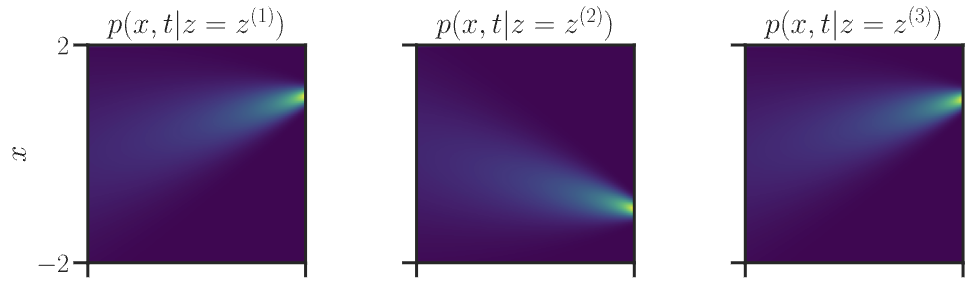
\includegraphics[width=\linewidth]{figs/conical_paths}
	\end{figure}
\end{frame}
%=======
\section{Latent Space Models}
%=======
\subsection{Score-Based Models}
%=======
\begin{frame}{Latent Space Models}
    \myfootnote{\href{https://arxiv.org/abs/2307.08698}{Dao Q. et al. Flow Matching in Latent Space, 2023} \\ \href{https://neurips2023-ldm-tutorial.github.io/}{NeurIPS 2023 Tutorial: Latent Diffusion Models: Is the Generative AI Revolution Happening in Latent Space?}}
		\vspace{-0.3cm}
	\begin{block}{Score-Based Models (Diffusion)}
		\vspace{-0.3cm}
		\begin{figure}
			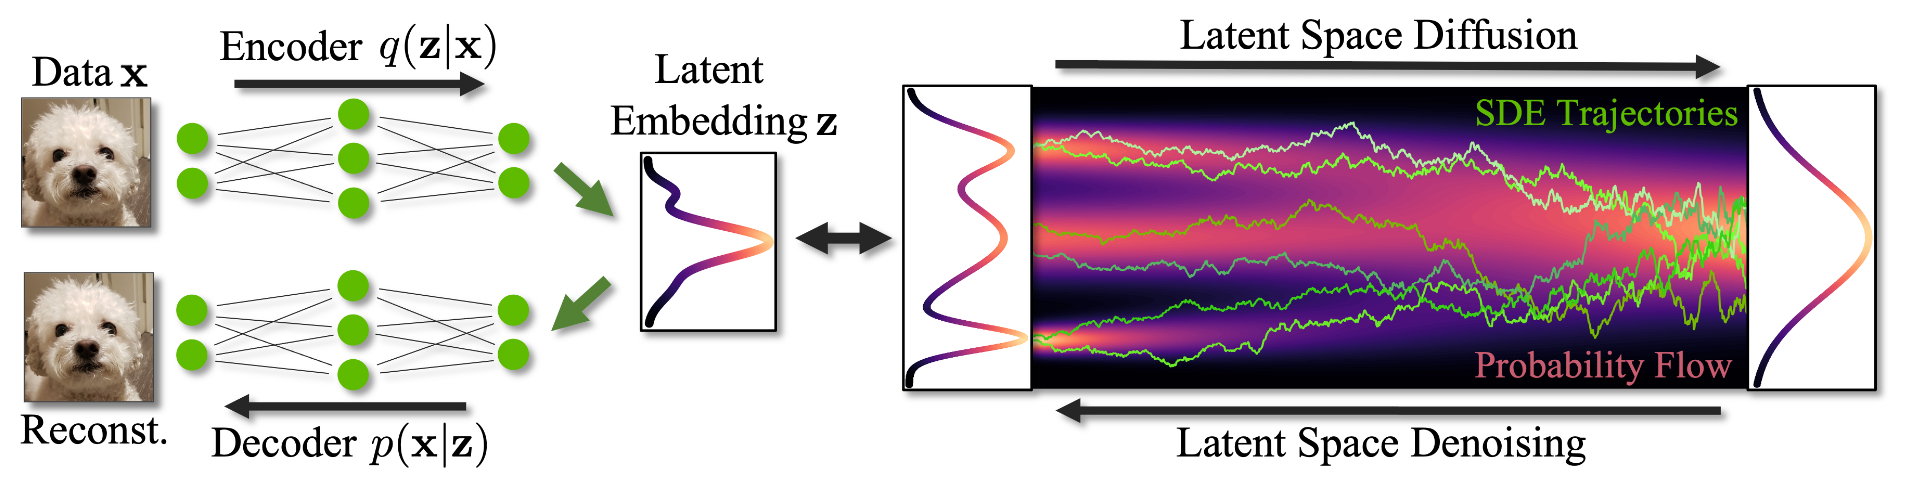
\includegraphics[width=\linewidth]{figs/latent_diffusion}
		\end{figure}
		\vspace{-0.3cm}
	\end{block}
	\begin{block}{Flow Matching}
		\vspace{-0.3cm}
		\begin{figure}
			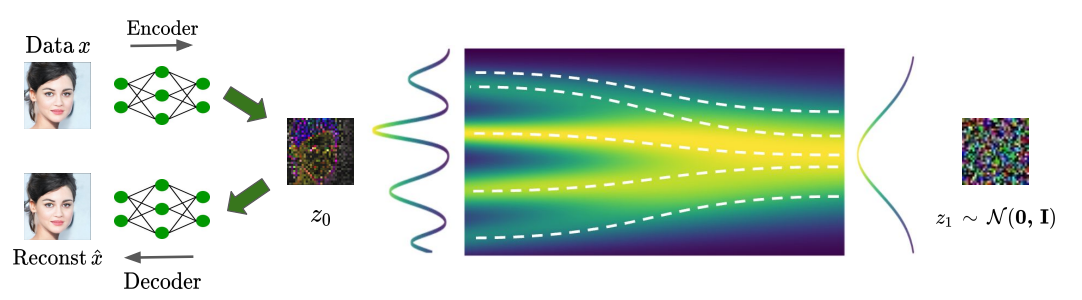
\includegraphics[width=\linewidth]{figs/latent_flow_matching}
		\end{figure}
	\end{block}
\end{frame}
%=======
\subsection{Autoregressive Models}
%=======
\begin{frame}{Vector Quantized VAE (VQ-VAE)}
    \myfootnote{\href{https://arxiv.org/abs/2004.02088}{Zhao Y. et al. Feature Quantization Improves GAN Training, 2020} \\ \href{https://arxiv.org/abs/1711.00937}{Oord A., Vinyals O., Kavukcuoglu K. Neural Discrete Representation Learning, 2017}}
	Define a dictionary space $\{\be_k\}_{k=1}^K$, where $\be_k \in \bbR^C$ and $K$ is the dictionary’s size.
	\vspace{-0.5cm}
	\begin{minipage}[t]{0.45\columnwidth}
		\[
			\bz_q = \bq (\bz) = \be_{k^*}
		\]
		Here $k^* = \argmin_k \| \bz - \be_k \|$.
	\end{minipage}%
	\begin{minipage}[t]{0.55\columnwidth}
		\vspace{-0.5cm}
		\begin{figure}
			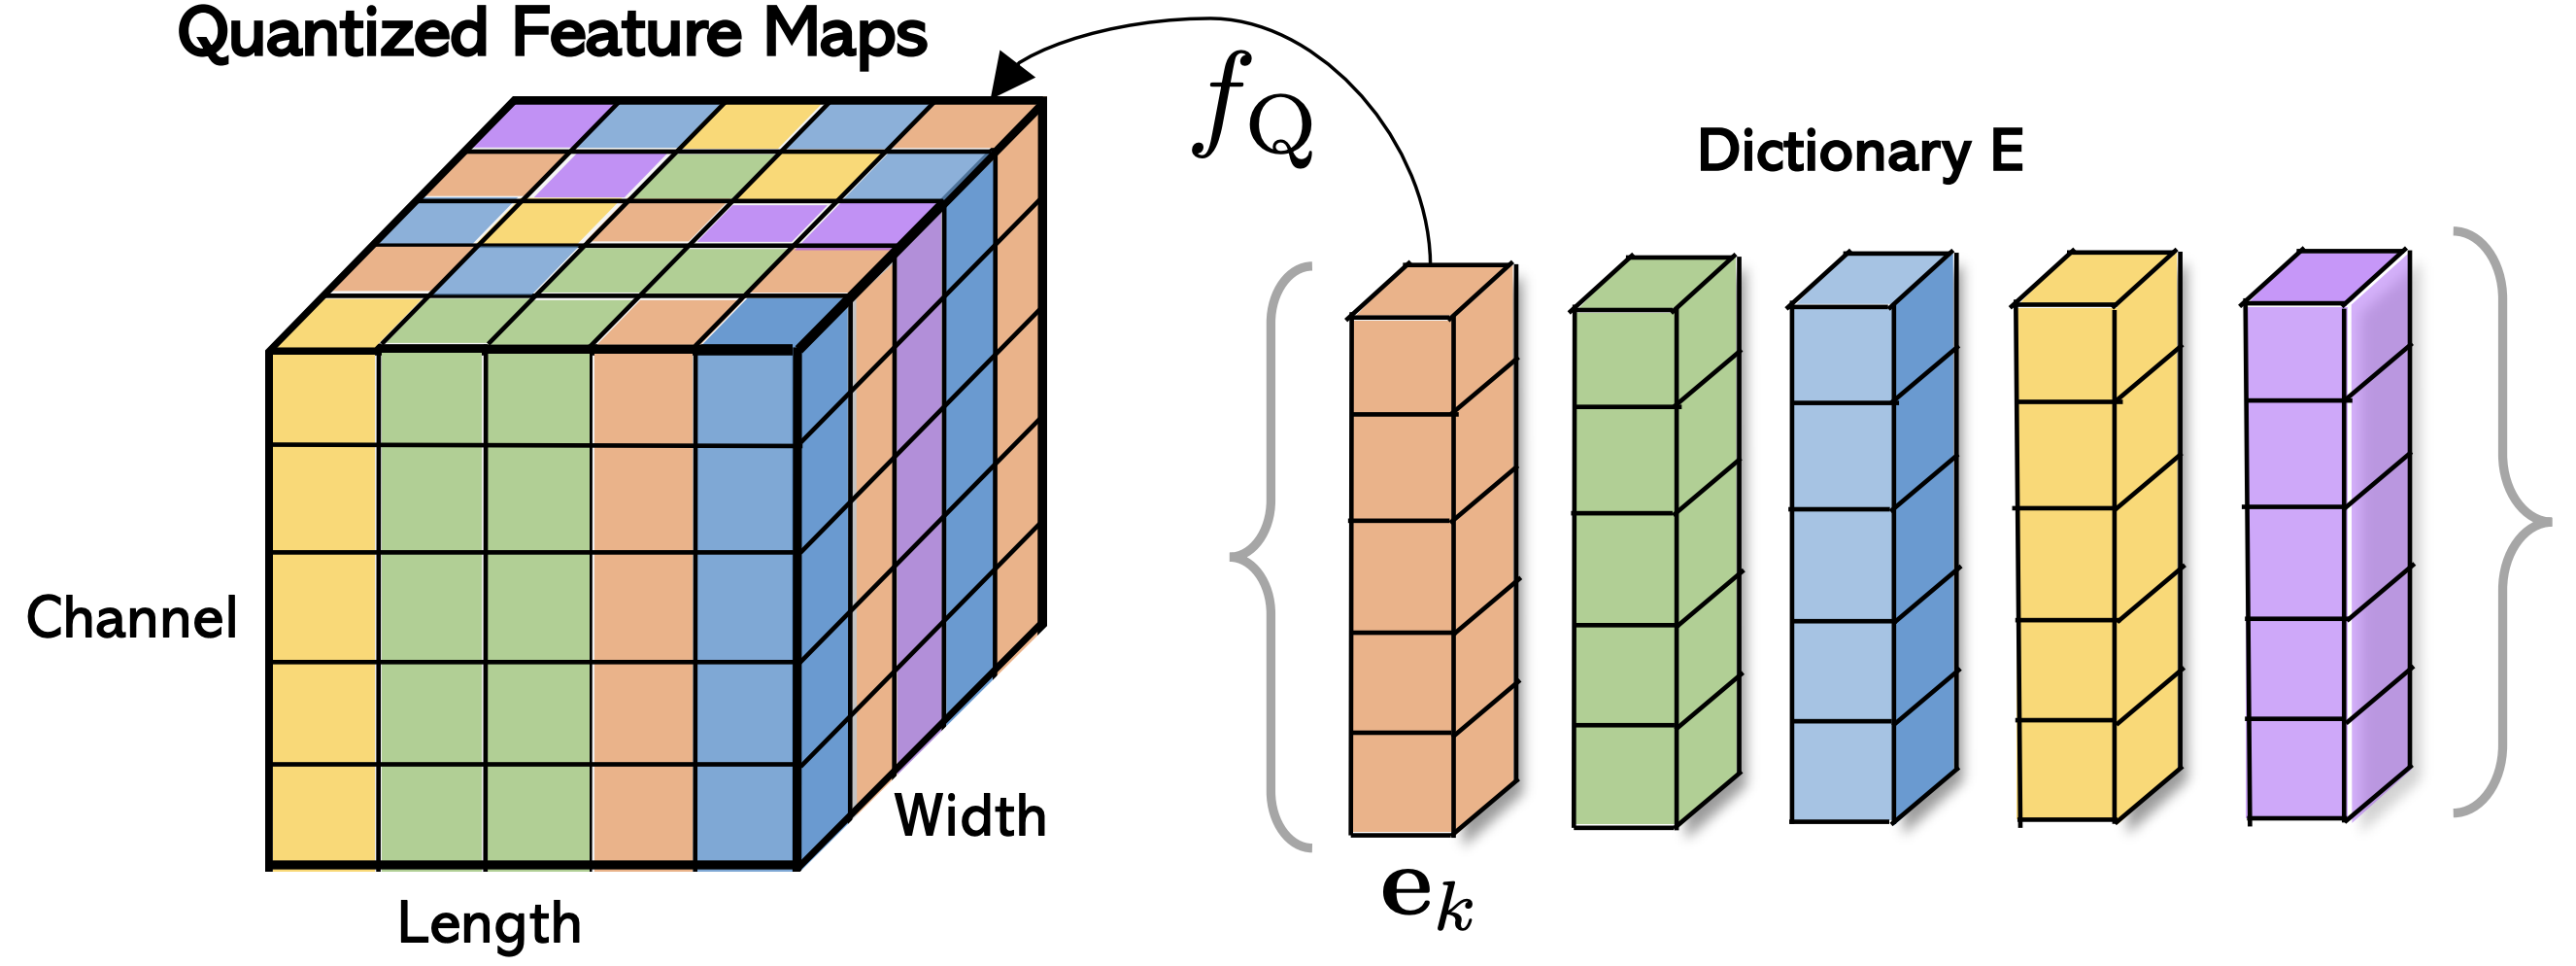
\includegraphics[width=\linewidth]{figs/fqgan_cnn}
		\end{figure}
	\end{minipage}		
	\[
		\cL_{\bphi, \btheta}(\bx)  =  \log p(\bx | \bz_q, \btheta) - \log K
	\]
	\vspace{-0.5cm}
	\begin{figure}
		\centering
		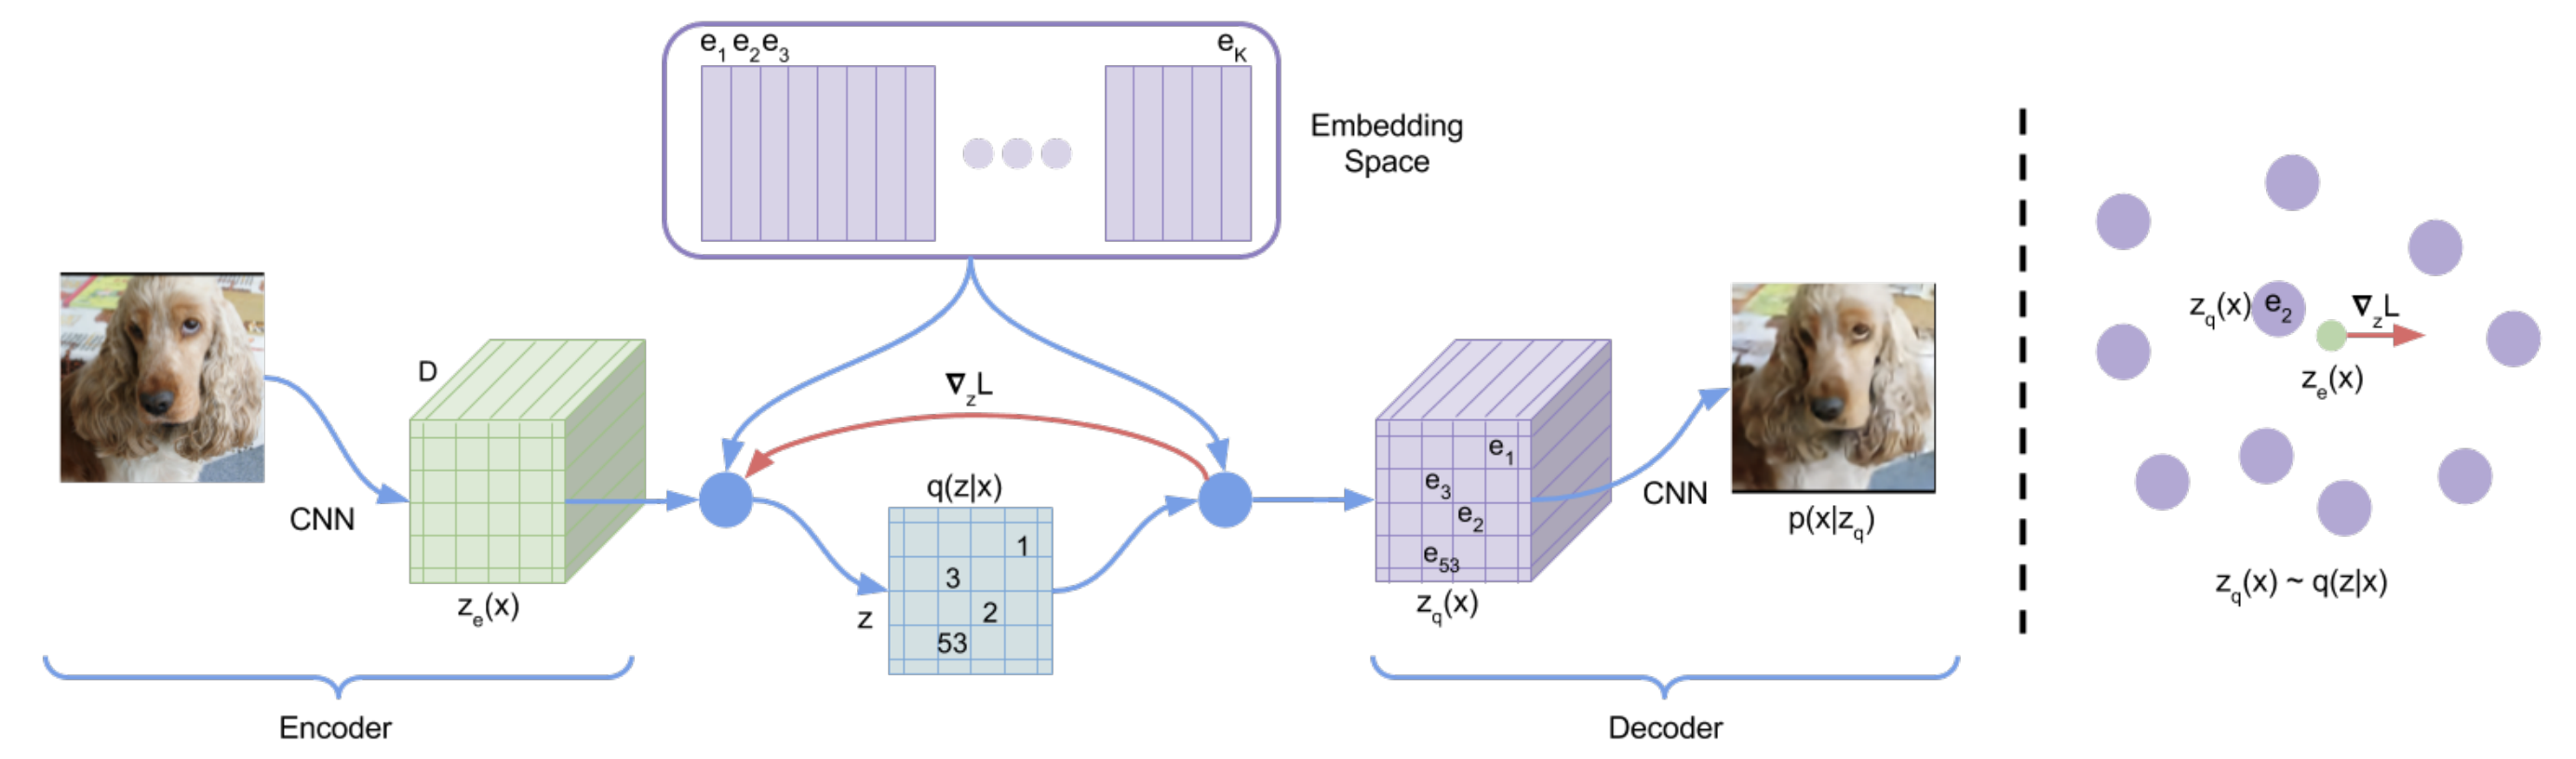
\includegraphics[width=\linewidth]{figs/vqvae}
	\end{figure}
\end{frame}
%=======
\begin{frame}{Vector Quantized GAN}
    \myfootnotewithlink{https://arxiv.org/abs/2012.09841}{Esser P. et al. Taming Transformers for High-Resolution Image Synthesis, 2020}
	\begin{itemize}
		\item We use a VQ-VAE model and its objective.
		\item We add an adversarial loss between generated and real images to further improve the visual quality of reconstructions.
	\end{itemize}
	\begin{figure}
		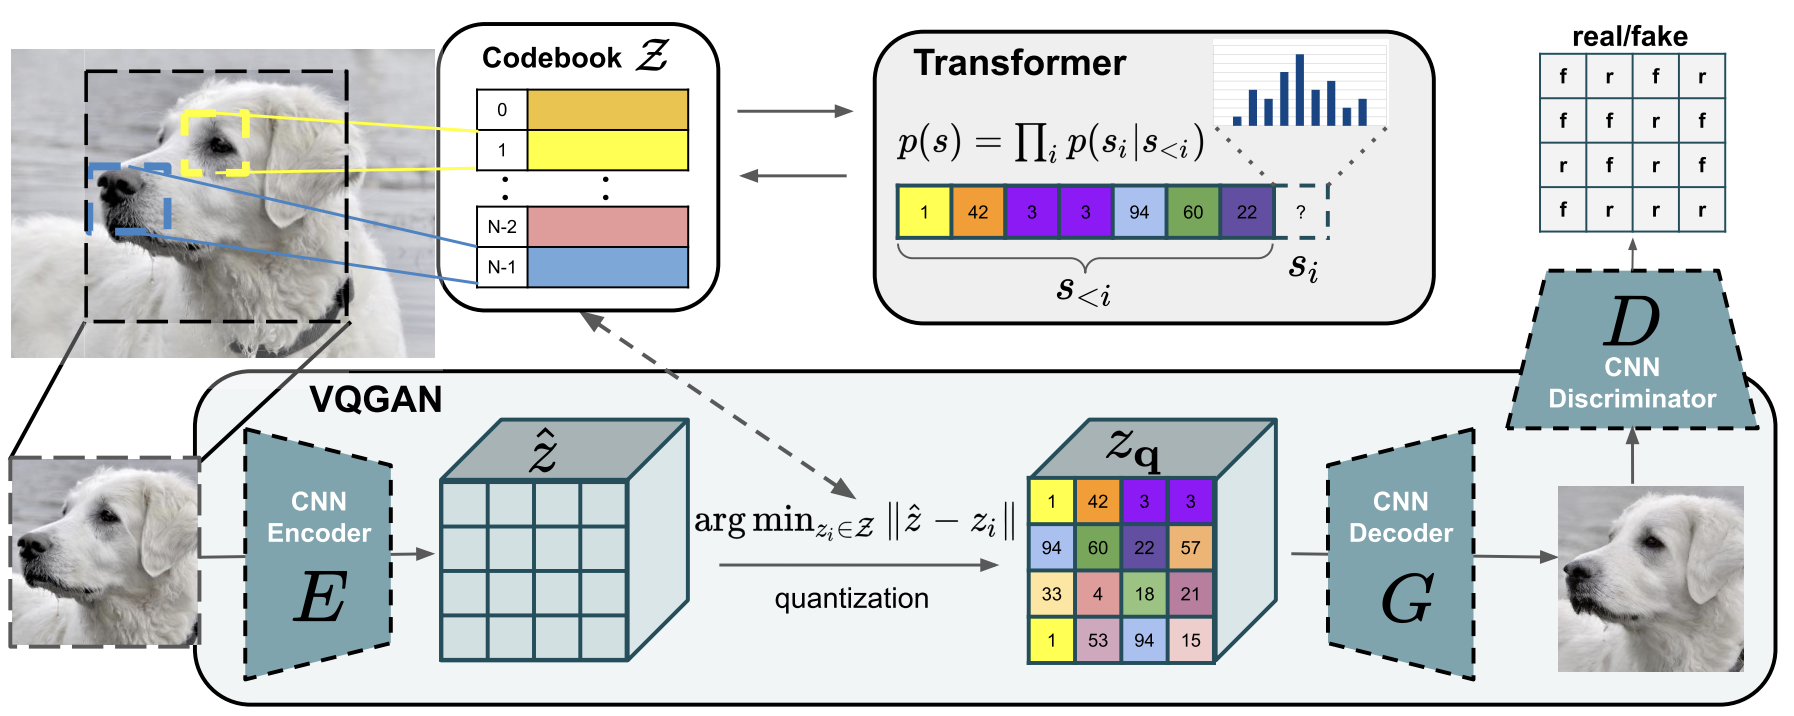
\includegraphics[width=\linewidth]{figs/vqgan}
	\end{figure}
\end{frame}
%=======
\begin{frame}{LlamaGen: Pure Autoregression}
    \myfootnotewithlink{https://arxiv.org/pdf/2406.06525}{Sun P. et al. Autoregressive Model Beats Diffusion: Llama for Scalable Image Generation, 2024}
	\begin{itemize}
		\item Use a VQ-GAN encoder for mapping images into the discrete latent space (codebook vectors).
		\item Train a pure autoregressive model (Llama-based) in the latent space.
		\item Use the VQ-GAN decoder to map discrete tokens back to image space.
	\end{itemize}
	\vspace{-0.3cm}
	\begin{figure}
		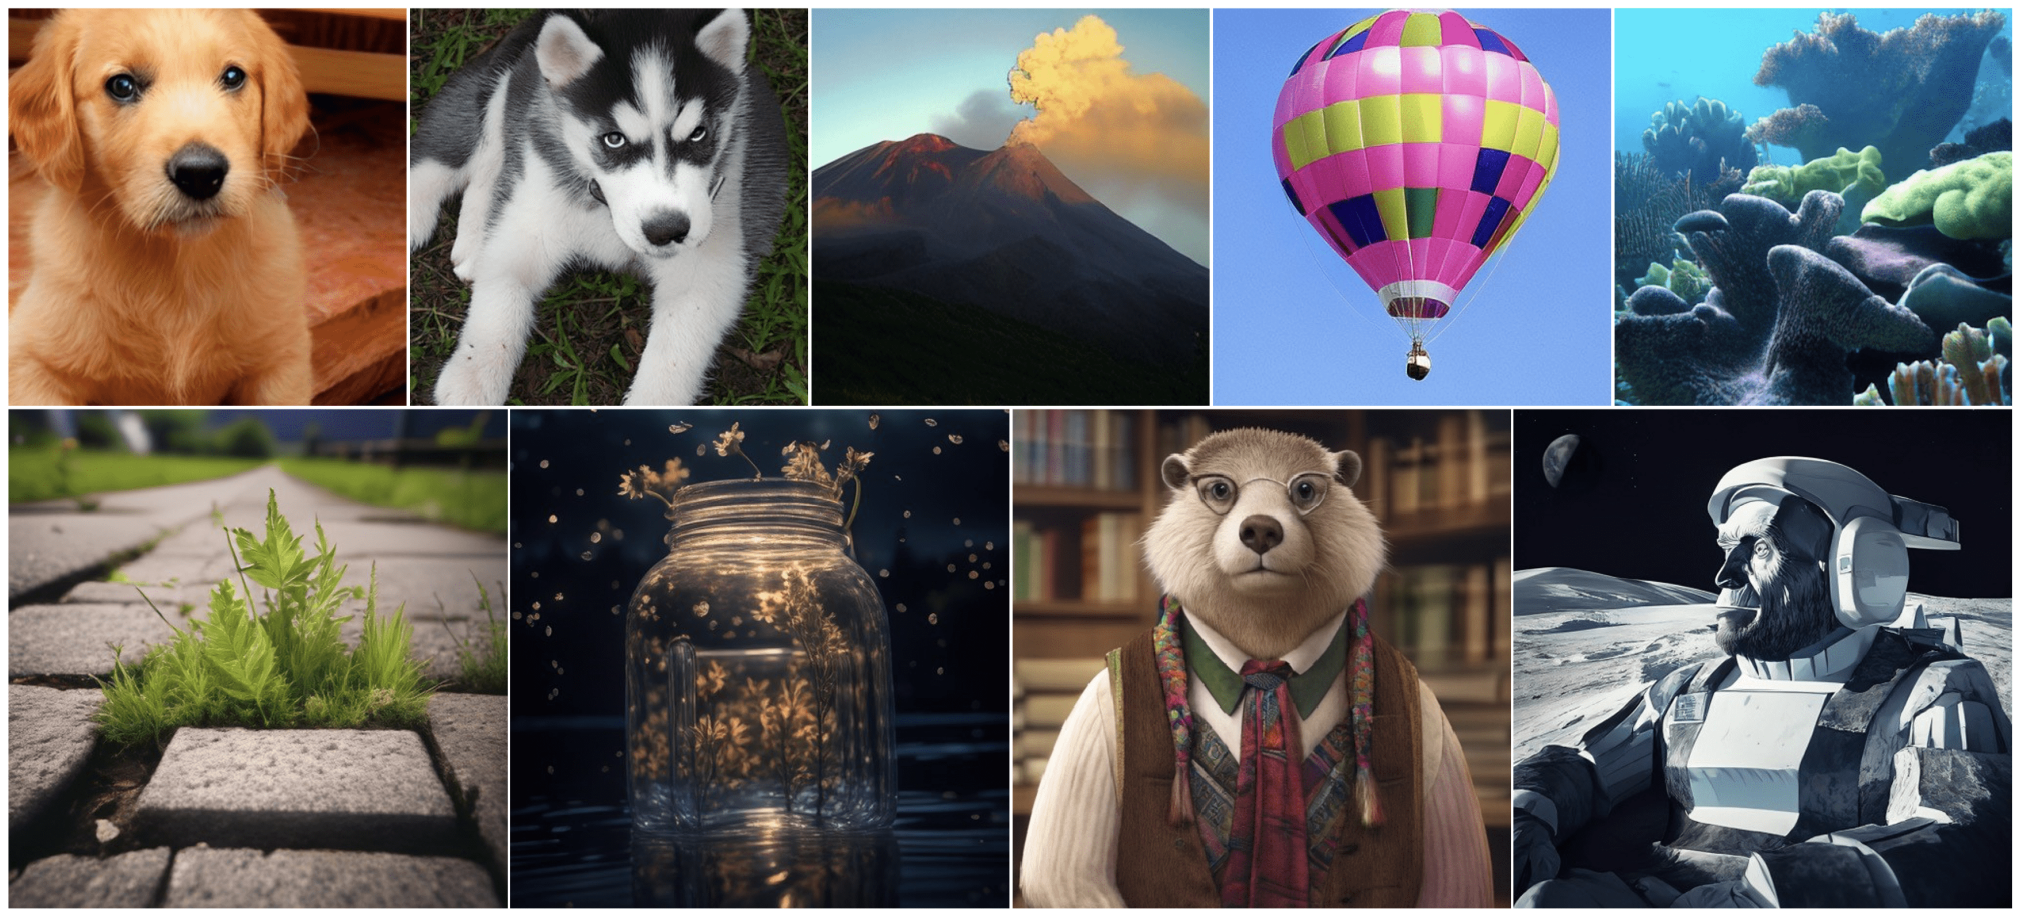
\includegraphics[width=0.85\linewidth]{figs/llamagen_samples}
	\end{figure}
\end{frame}
%=======
\begin{frame}{Visual Autoregressive Modeling (VAR)}
    \myfootnotewithlink{https://arxiv.org/pdf/2404.02905}{Tean K. et al. Visual Autoregressive Modeling: Scalable Image Generation via Next-Scale Prediction, 2024}
	\begin{figure}
		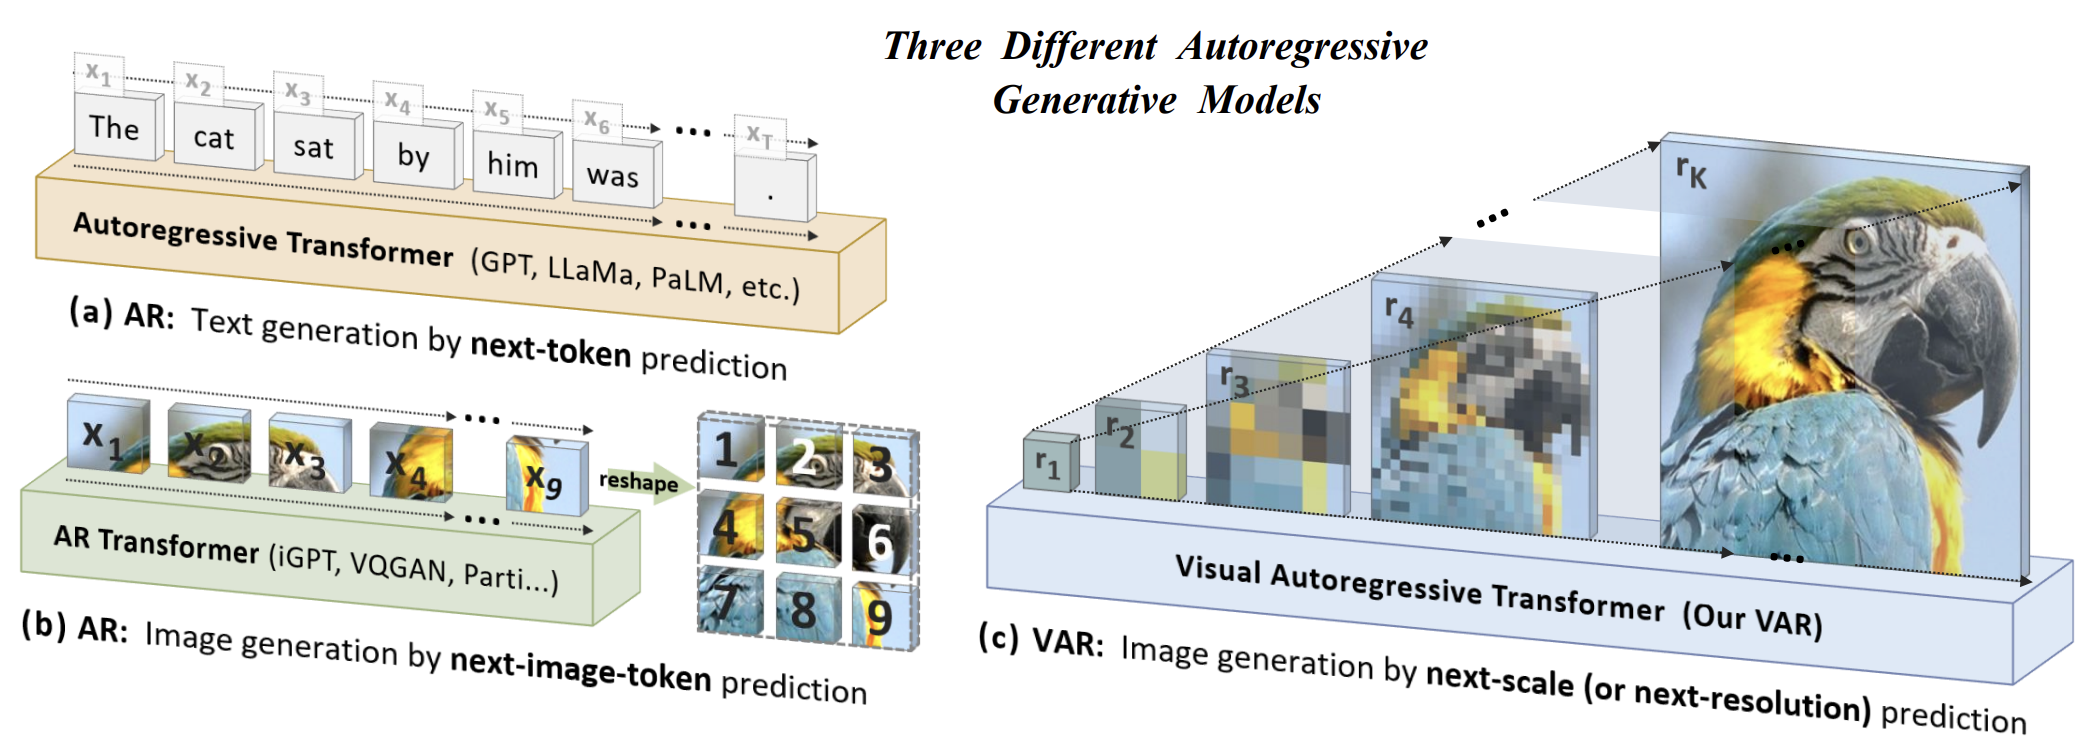
\includegraphics[width=0.9\linewidth]{figs/var_idea}
	\end{figure}
	\begin{figure}
		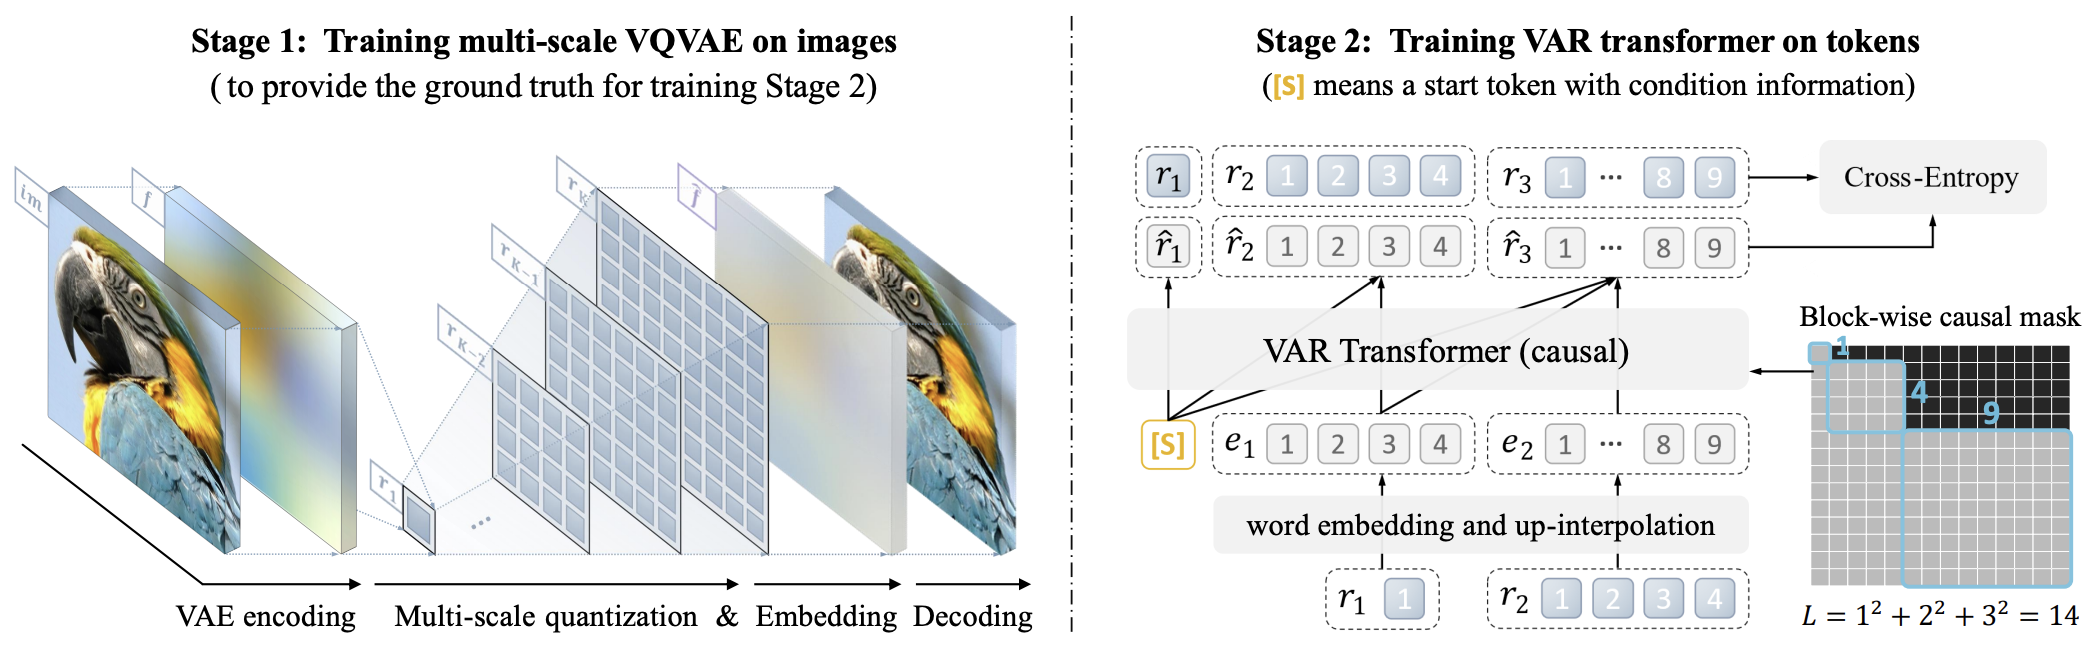
\includegraphics[width=0.9\linewidth]{figs/var_training}
	\end{figure}
\end{frame}
%=======
\section{The Worst Course Overview}
%=======
\begin{frame}{The Worst Course Overview :)}
    \myfootnotewithlink{https://lilianweng.github.io/posts/2021-07-11-diffusion-models/}{Weng L. What are Diffusion Models?, blog post, 2021}
	\begin{figure}
		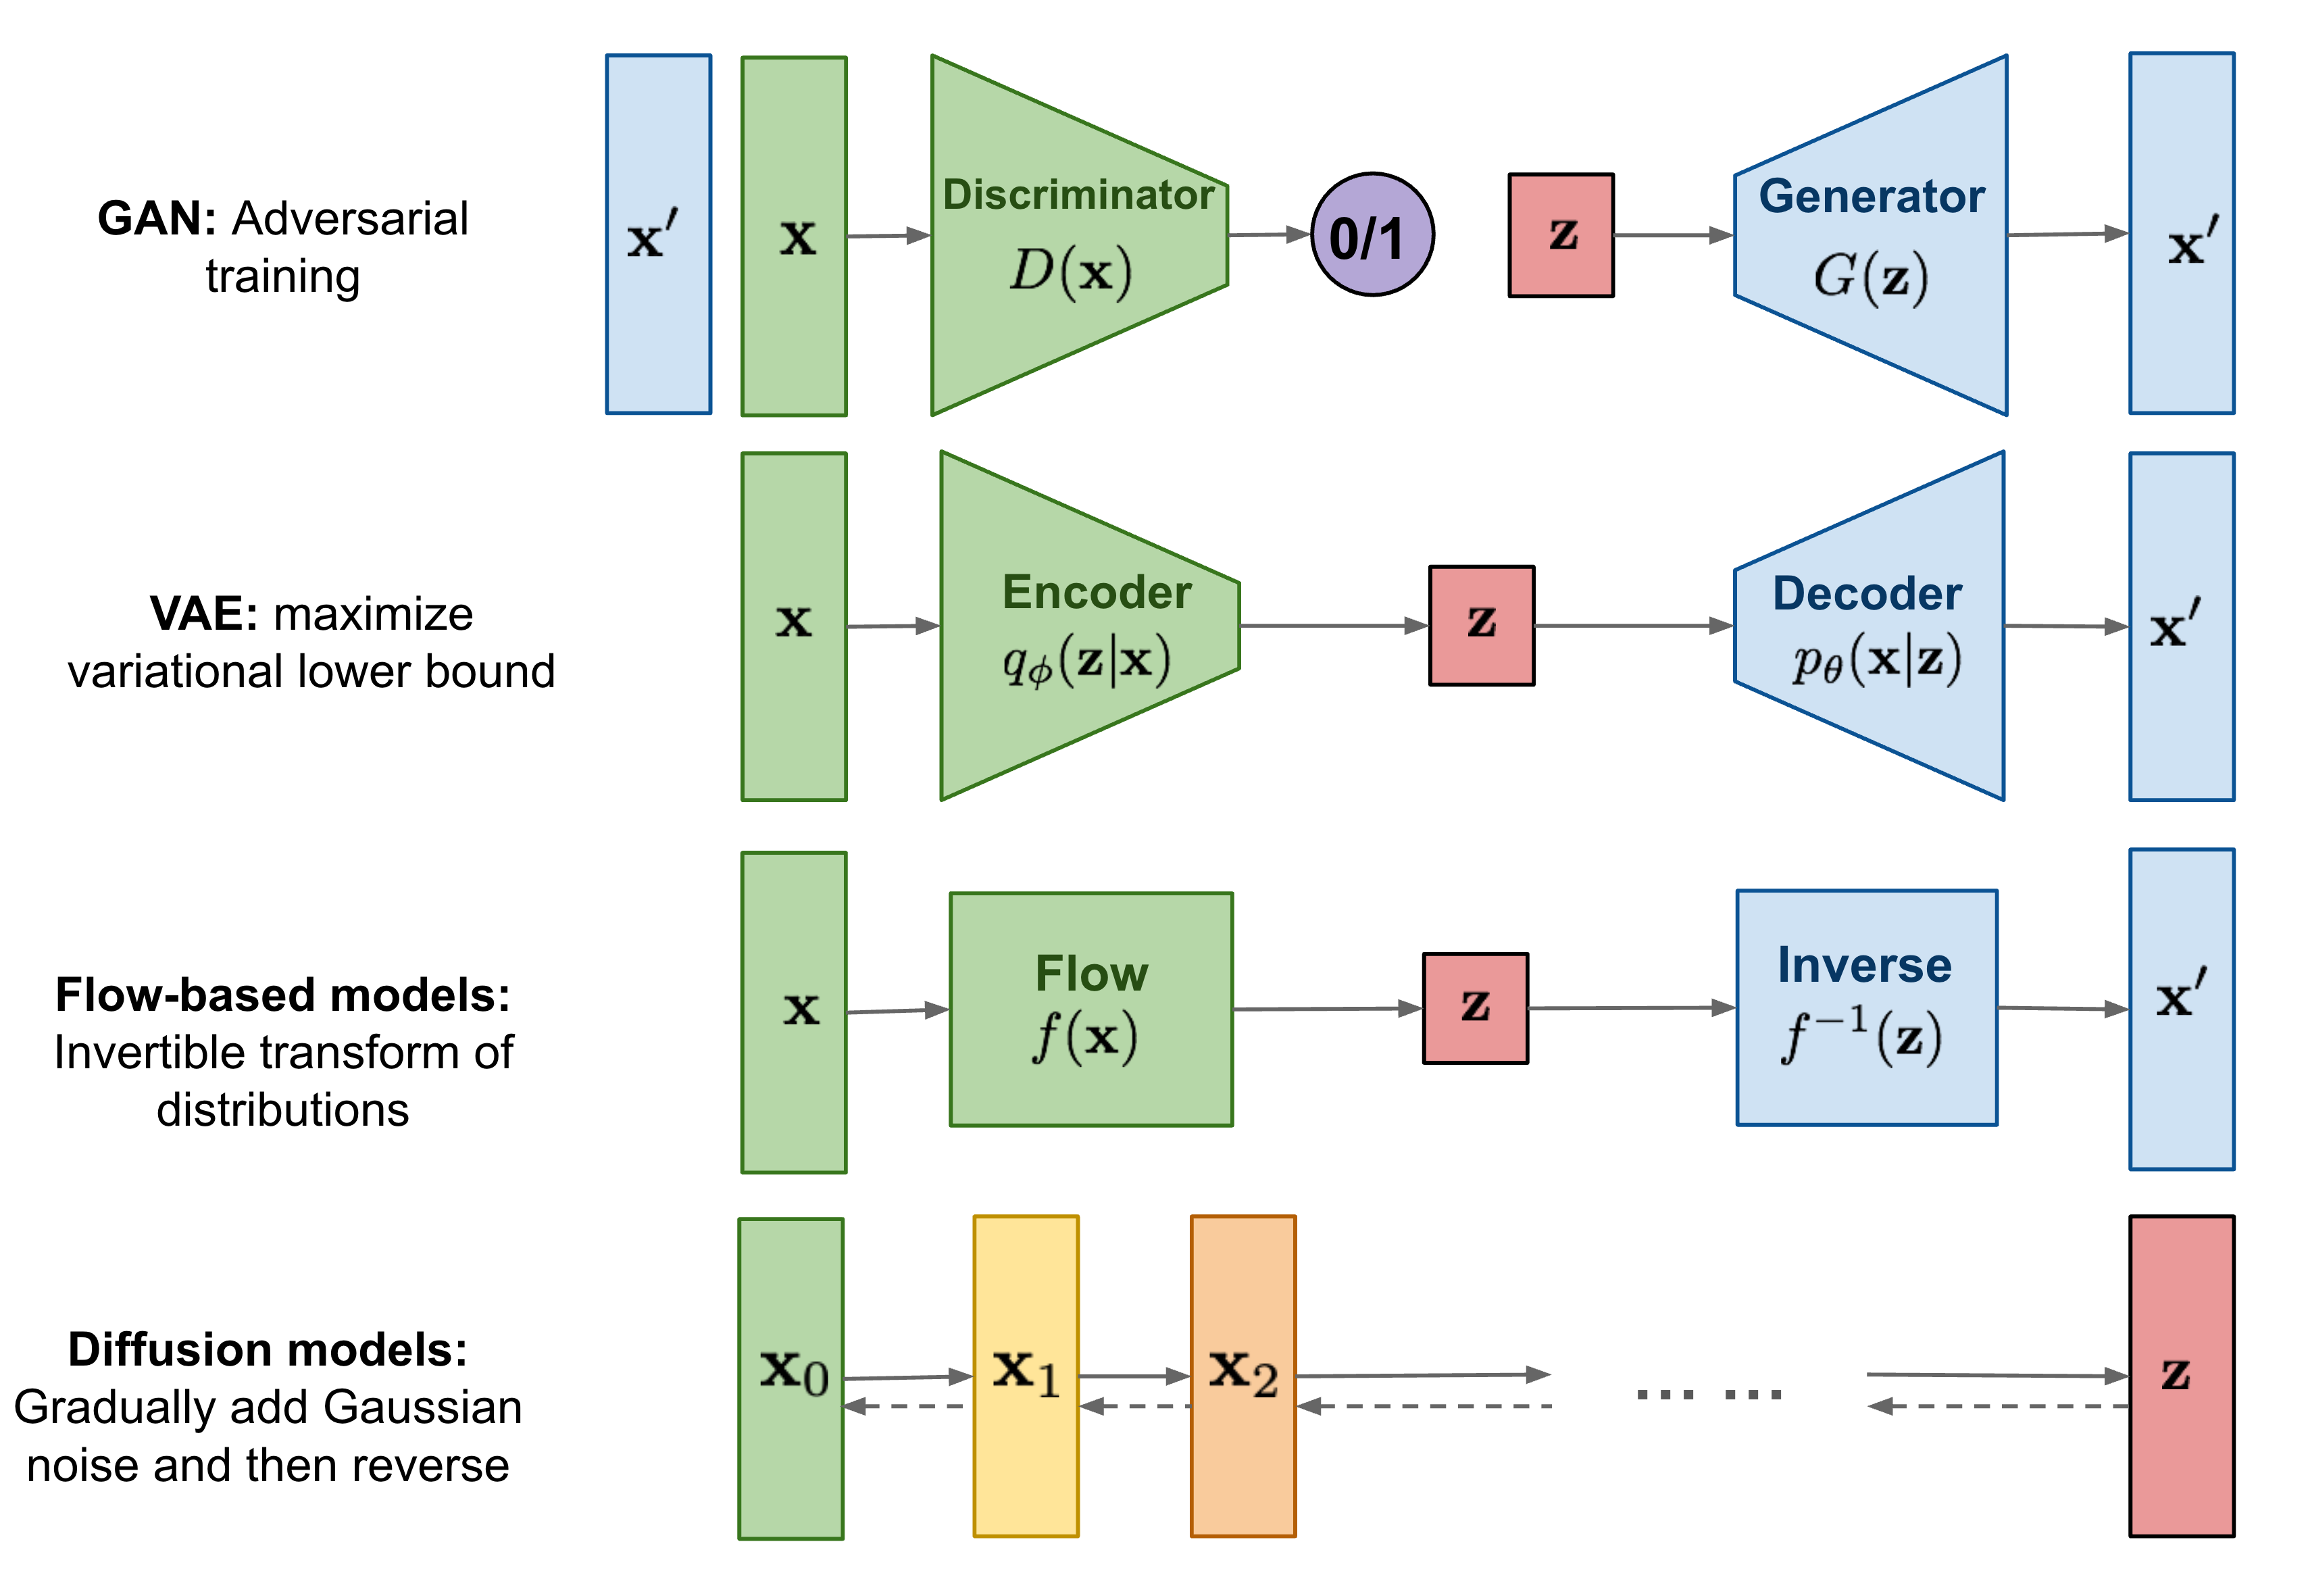
\includegraphics[width=\linewidth]{figs/generative-overview}
	\end{figure}
\end{frame}
%=======
\begin{frame}{The Worst Course Overview :)}
    \myfootnote{\href{https://arxiv.org/abs/2112.07804}{Xiao Z., Kreis K., Vahdat A. Tackling the generative learning trilemma with denoising diffusion GANs, 2021} \\ \href{https://udlbook.github.io/udlbook/}{Simon J.D. Prince. Understanding Deep Learning, 2023}}
	\vspace{-0.3cm}
	\begin{figure}
		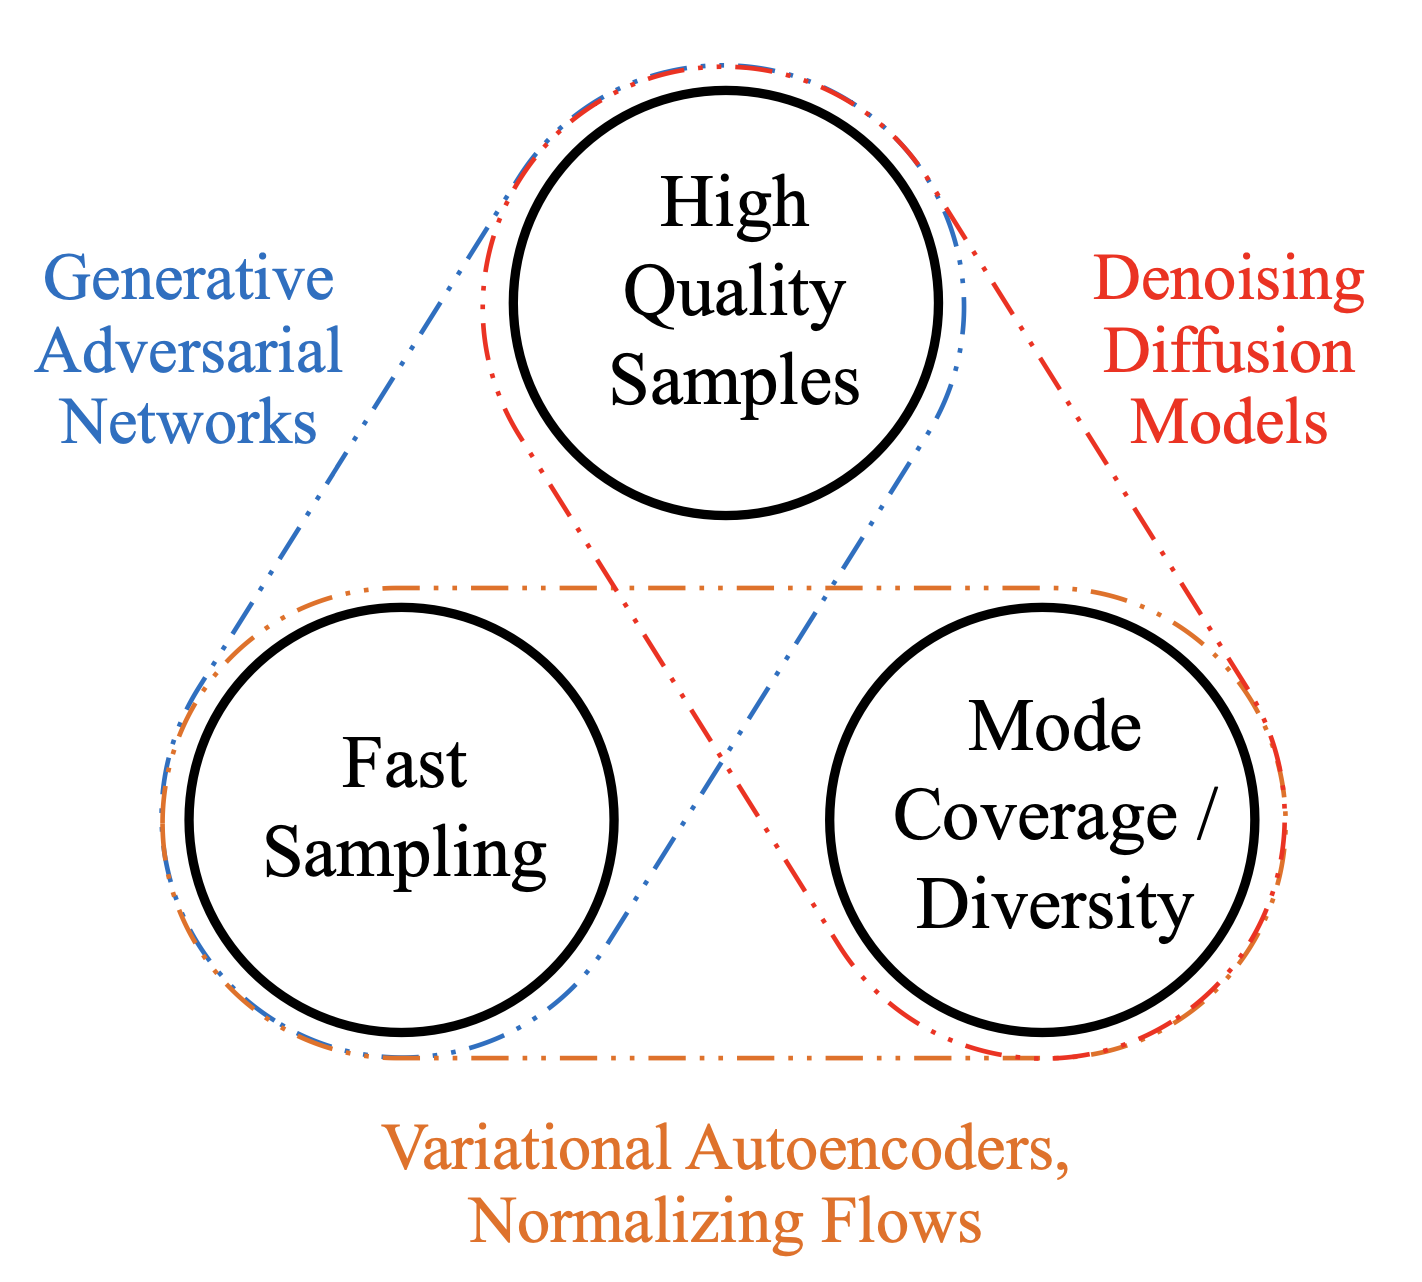
\includegraphics[width=0.45\linewidth]{figs/trilemma}
	\end{figure}
	\vspace{-0.5cm}
	\begin{figure}
		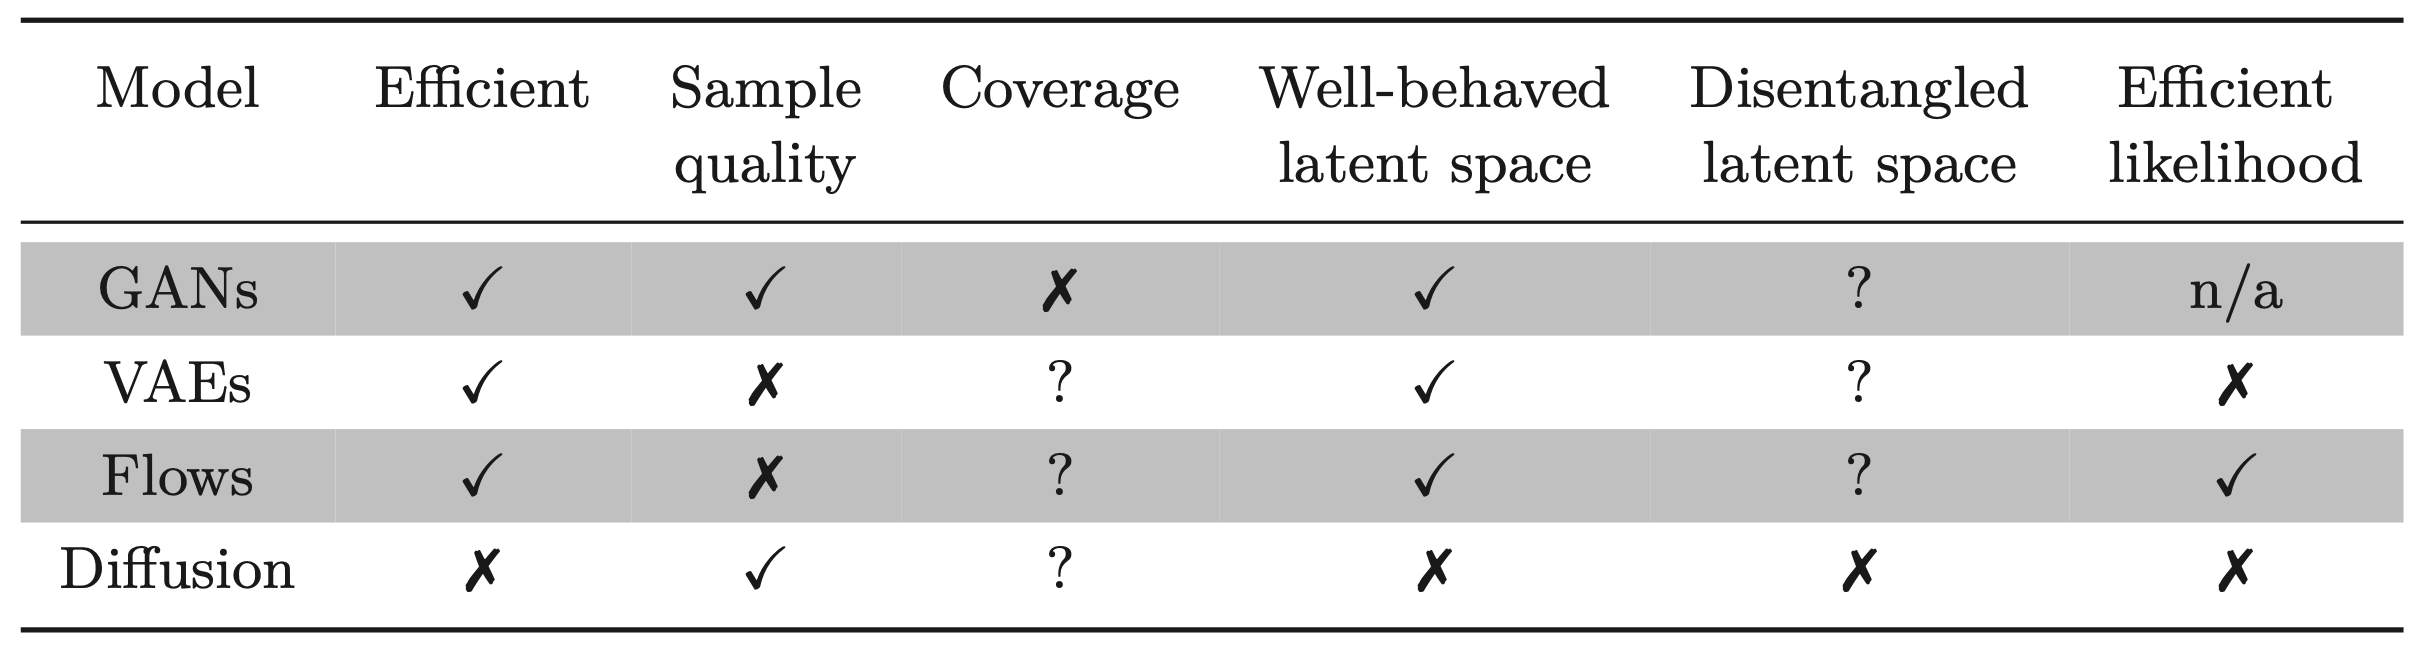
\includegraphics[width=0.9\linewidth]{figs/gen_comp_table}
	\end{figure}
\end{frame}
%=======
\begin{frame}{Summary}
	\begin{itemize}
		\item Most state-of-the-art generative models are latent variable models with either continuous or discrete latent spaces.
	\end{itemize}
\end{frame}
\end{document}